\documentclass[tikz,border=0pt]{standalone}

\usepackage[T1]{fontenc}
\usepackage{newtxtext}
\usepackage{newtxmath}
\usepackage{xcolor}
\usetikzlibrary{positioning}

\definecolor{estone}{HTML}{1B7837}
\definecolor{esttwo}{HTML}{4DAF4A}
\definecolor{estthree}{HTML}{A6D96A}
\definecolor{validblue}{HTML}{2C7FB8}
\definecolor{ignoredgray}{HTML}{BDBDBD}
\definecolor{gridgray}{HTML}{ECECEC}
\definecolor{textgray}{HTML}{303030}
\definecolor{bandgray}{HTML}{F5F5F5}

\pagecolor{white}

\newcommand{\funddot}[3]{%
	\filldraw[fill=#3, draw=white, line width=0.35pt] (#1,#2) circle[radius=2.2pt];
}

\begin{document}
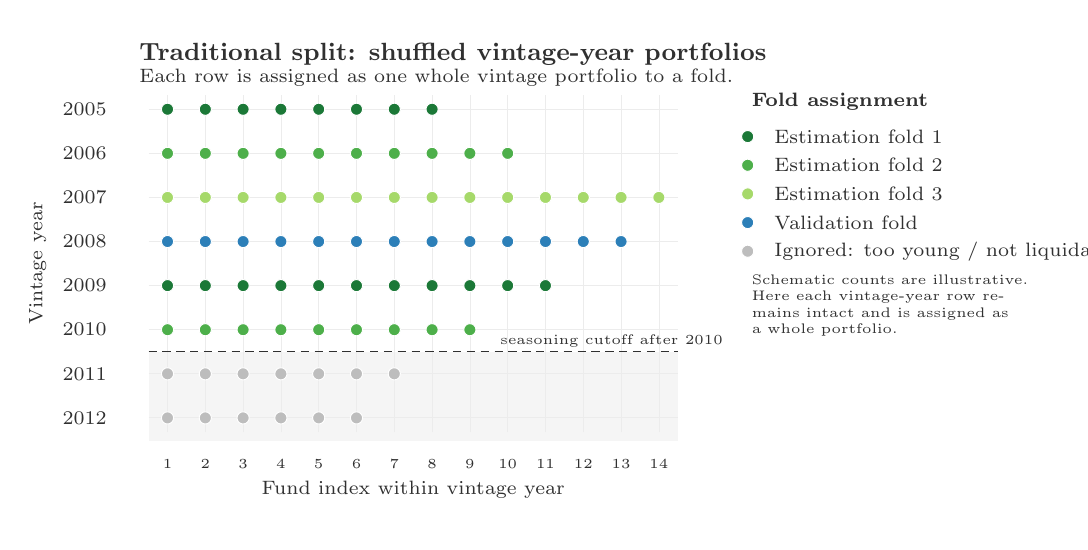
\begin{tikzpicture}[x=0.48cm,y=0.56cm]
	% Fixed white canvas so PDF-to-PNG conversion never creates a transparent margin.
	\path[use as bounding box] (-2.7,-9.35) rectangle (24.6,1.85);
	\fill[white] (-2.7,-9.35) rectangle (24.6,1.85);

	% Compact panel title. The paper caption should carry the full methodological text.
	\node[anchor=west, font=\bfseries\small, text=textgray] at (0,1.25)
		{Traditional split: shuffled vintage-year portfolios};
	\node[anchor=west, font=\scriptsize, text=textgray] at (0,0.72)
		{Each row is assigned as one whole vintage portfolio to a fold.};

	% Light background for young vintages excluded from estimation and validation.
	\fill[bandgray] (0.5,-5.5) rectangle (14.5,-7.52);

	% Grid and y-axis labels.
	\foreach \y/\year in {0/2005,-1/2006,-2/2007,-3/2008,-4/2009,-5/2010,-6/2011,-7/2012} {
		\draw[gridgray, line width=0.3pt] (0.5,\y) -- (14.5,\y);
		\node[anchor=east, font=\scriptsize, text=textgray] at (-0.35,\y) {\year};
	}

	% x-axis labels and faint vertical guides.
	\foreach \x in {1,...,14} {
		\draw[gridgray, line width=0.22pt] (\x,-7.32) -- (\x,0.32);
		\node[anchor=north, font=\tiny, text=textgray] at (\x,-7.72) {\x};
	}
	\node[anchor=north, font=\scriptsize, text=textgray] at (7.5,-8.2)
		{Fund index within vintage year};
	\node[rotate=90, anchor=south, font=\scriptsize, text=textgray] at (-1.95,-3.5)
		{Vintage year};

	% Whole-vintage portfolio assignments.
	\foreach \x in {1,...,8} {\funddot{\x}{0}{estone}}
	\foreach \x in {1,...,10} {\funddot{\x}{-1}{esttwo}}
	\foreach \x in {1,...,14} {\funddot{\x}{-2}{estthree}}
	\foreach \x in {1,...,13} {\funddot{\x}{-3}{validblue}}
	\foreach \x in {1,...,11} {\funddot{\x}{-4}{estone}}
	\foreach \x in {1,...,9} {\funddot{\x}{-5}{esttwo}}

	% 2011 and 2012: ignored because these vintages are too young / not liquidated enough.
	\foreach \x in {1,...,7} {\funddot{\x}{-6}{ignoredgray}}
	\foreach \x in {1,...,6} {\funddot{\x}{-7}{ignoredgray}}

	% Cutoff annotation.
	\draw[densely dashed, textgray, line width=0.35pt] (0.5,-5.5) -- (14.5,-5.5);
	\node[anchor=west, font=\tiny, text=textgray] at (9.55,-5.25)
		{seasoning cutoff after 2010};

	% Legend, placed to the right to avoid crowding the x-axis.
	\node[anchor=west, font=\bfseries\scriptsize, text=textgray] at (16.2,0.18)
		{Fold assignment};
	\funddot{16.35}{-0.62}{estone}
	\node[anchor=west, font=\scriptsize, text=textgray] at (16.8,-0.62)
		{Estimation fold 1};
	\funddot{16.35}{-1.27}{esttwo}
	\node[anchor=west, font=\scriptsize, text=textgray] at (16.8,-1.27)
		{Estimation fold 2};
	\funddot{16.35}{-1.92}{estthree}
	\node[anchor=west, font=\scriptsize, text=textgray] at (16.8,-1.92)
		{Estimation fold 3};
	\funddot{16.35}{-2.57}{validblue}
	\node[anchor=west, font=\scriptsize, text=textgray] at (16.8,-2.57)
		{Validation fold};
	\funddot{16.35}{-3.22}{ignoredgray}
	\node[anchor=west, font=\scriptsize, text=textgray] at (16.8,-3.22)
		{Ignored: too young / not liquidated};

	\node[anchor=west, align=left, text width=3.7cm, font=\tiny, text=textgray] at (16.2,-4.45)
		{Schematic counts are illustrative. Here each vintage-year row remains intact and is assigned as a whole portfolio.};
\end{tikzpicture}
\end{document}
